\subsubsection{Neural Autoencoders}\label{sec:neural-autoencoders}

Before studying \textbf{word embeddings}, it is useful to understand the idea of an \textbf{autoencoder}, because it represents one of the most important examples of unsupervised representation learning. In fact, the central \textbf{goal of both autoencoders and word embeddings is the same}: \hl{learn a compact and meaningful representation of data without requiring labels.}

\highspace
\begin{flushleft}
    \textcolor{Green3}{\faIcon{tools} \textbf{Autoencoder Architecture}}
\end{flushleft}
A \definition{Neural Autoencoder} is a \textbf{neural network trained to reproduce its input at the output}:
\begin{equation*}
    g(x) \approx x
\end{equation*}
In other words, the network is asked to learn the identity function. At first sight this might seem pointless: \emph{\textbf{if the desired output is exactly the input, why not simply copy it?}} The answer is that we \hl{deliberately constrain the network so that copying becomes impossible.} Let's see how.

\highspace
The typical architecture (see \autoref{fig:autoencoder}, \autopageref{fig:autoencoder}) is composed of \textbf{three parts}:
\begin{equation*}
    x \xrightarrow{\text{Encoder}} h \xrightarrow{\text{Decoder}} g
\end{equation*}
Where:
\begin{itemize}
    \item $x \in \mathbb{R}^{I}$ is the \textbf{input} vector;
    \item $h \in \mathbb{R}^{J}$ is the \textbf{hidden representation} (or \textbf{latent code});
    \item $g \in \mathbb{R}^{I}$ is the \textbf{reconstructed} output vector.
\end{itemize}
Usually, the input and output dimensions are the same ($\mathbb{R}^{I}$), while the hidden representation is much smaller ($\mathbb{R}^{J}$): $J \ll I$. It means that the hidden layer contains far fewer neurons than the input layer. This creates a \textbf{bottleneck}, \hl{forcing the network to compress the information contained in the input.}

\highspace
\textcolor{Green3}{\faIcon{compress}} The \textbf{encoder} transforms the original data into a compact \textbf{latent representation}:
\begin{equation}\label{eq:auto-encoder}
    h = \mathrm{enc}(x)
\end{equation}
This \hl{latent vector} should \hl{contain only the most relevant information needed to describe the input.} \textcolor{Green3}{\faIcon{reply}} The \textbf{decoder} then reconstructs the \textbf{original sample} from this compressed representation:
\begin{equation}\label{eq:auto-decoder}
    g = \mathrm{dec}(h)
\end{equation}
The complete network can therefore be written as:
\begin{equation}
    g = \mathrm{dec}(\underbrace{\mathrm{enc}(x)}_{h})
\end{equation}
The \textbf{encoder} can be viewed as a \textbf{compression} mechanism, while the \textbf{decoder} acts as a \textbf{decompression} mechanism. Together they \hl{learn how to represent the input efficiently.}

\begin{figure}[!htp]
    \centering
    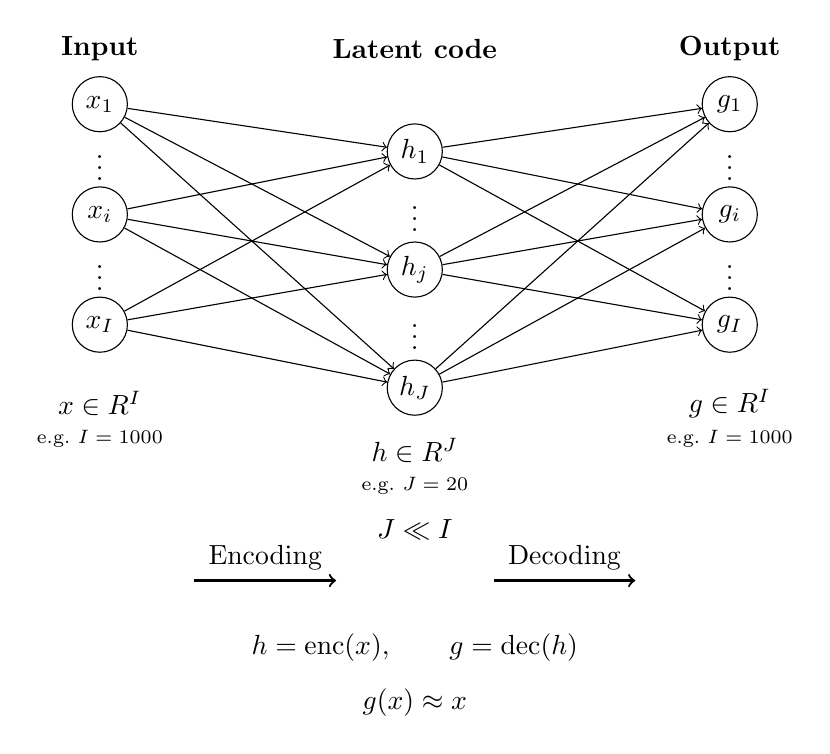
\begin{tikzpicture}[
        neuron/.style={circle, draw, minimum size=7mm, inner sep=0pt},
        layerlabel/.style={font=\bfseries},
        arrow/.style={->, thick}
    ]
        % Input layer
        \node[neuron] (x1) at (0,  1.6) {$x_1$};
        \node at (0,  0.9) {$\vdots$};
        \node[neuron] (xi) at (0,  0.2) {$x_i$};
        \node at (0, -0.5) {$\vdots$};
        \node[neuron] (xI) at (0, -1.2) {$x_I$};

        % Latent layer
        \node[neuron] (h1) at (4,  1.0) {$h_1$};
        \node at (4,  0.25) {$\vdots$};
        \node[neuron] (hj) at (4, -0.5) {$h_j$};
        \node at (4, -1.25) {$\vdots$};
        \node[neuron] (hJ) at (4, -2.0) {$h_J$};

        % Output layer
        \node[neuron] (g1) at (8,  1.6) {$g_1$};
        \node at (8,  0.9) {$\vdots$};
        \node[neuron] (gi) at (8,  0.2) {$g_i$};
        \node at (8, -0.5) {$\vdots$};
        \node[neuron] (gI) at (8, -1.2) {$g_I$};

        % Connections
        \foreach \x in {x1,xi,xI}
        \foreach \h in {h1,hj,hJ}
            \draw[->, thin] (\x) -- (\h);

        \foreach \h in {h1,hj,hJ}
        \foreach \g in {g1,gi,gI}
            \draw[->, thin] (\h) -- (\g);

        % Layer titles
        \node[layerlabel] at (0, 2.3) {Input};
        \node[layerlabel] at (4, 2.3) {Latent code};
        \node[layerlabel] at (8, 2.3) {Output};

        % Dimension labels
        \node at (0, -2.2) {$x \in \mathbb{R}^{I}$};
        \node at (0, -2.65) {\scriptsize e.g.\ $I=1000$};

        \node at (4, -2.8) {$h \in \mathbb{R}^{J}$};
        \node at (4, -3.25) {\scriptsize e.g.\ $J=20$};

        \node at (8, -2.2) {$g \in \mathbb{R}^{I}$};
        \node at (8, -2.65) {\scriptsize e.g.\ $I=1000$};

        \node at (4, -3.8) {$J \ll I$};

        % Encoding / Decoding arrows
        \draw[arrow] (1.2, -4.45) -- node[above] {Encoding} (3.0, -4.45);
        \draw[arrow] (5.0, -4.45) -- node[above] {Decoding} (6.8, -4.45);

        % Mapping equations
        \node at (4, -5.3)
        {$h = \mathrm{enc}(x), \qquad g = \mathrm{dec}(h)$};

        \node at (4, -6.0)
        {$g(x) \approx x$};
    \end{tikzpicture}
    \caption{Architecture of a neural autoencoder. The encoder compresses the input vector $x \in \mathbb{R}^{I}$ into a low-dimensional latent representation $h \in \mathbb{R}^{J}$ (where $J \ll I$), while the decoder reconstructs the original input, producing $g(x) \approx x$.}
    \label{fig:autoencoder}
\end{figure}

\highspace
\begin{flushleft}
    \textcolor{Red2}{\faIcon{exclamation-triangle} \textbf{Reconstruction Error}}
\end{flushleft}
Since the objective is to reconstruct the input, the \hl{network is trained by minimizing the difference between the original input and its reconstruction.} This difference is quantified by a \textbf{loss function}, which measures the \definition{Reconstruction Error}. The training process adjusts the parameters of both the encoder and decoder to minimize this error across the training dataset.

\highspace
A common loss function is the \textbf{squared reconstruction error}:
\begin{equation}
    E_{\text{rec}} = \sum_{i} \left(g_{i}(x) - x_i\right)^{2}
\end{equation}
This quantity measures \hl{how much information is lost during compression and reconstruction.} If the reconstruction error is \textbf{small}, the latent representation $h$ has \textbf{successfully captured the essential characteristics of the input}.

\highspace
The network therefore learns a representation that \textbf{preserves as much useful information as possible while using fewer dimensions}.

\newpage

\begin{flushleft}
    \textcolor{Green3}{\faIcon{question-circle} \textbf{Are there other ways to force compression?}}\phantomsection\label{def:dense-vector-representation}
\end{flushleft}
Reducing the size of the hidden layer is not the only way to force compression. Another common strategy is to impose a \textbf{sparsity constraint}.

\highspace
The idea is that only a \hl{small number of hidden neurons should be active for any given input}: $h_j \approx 0$ for most hidden units $j$. But, \emph{\textbf{how can we enforce this sparsity?}} First of all, with \emph{sparsity} we refer to the \textbf{latent representation} $h$. Suppose the encoder produces a vector $h$:
\begin{equation*}
    h = \left(h_1, h_2, \ldots, h_6\right)
\end{equation*}
Without any sparsity constraint, an input might produce a dense representation like:
\begin{equation*}
    h = \left(0.8, 0.6, 0.9, 0.7, 0.5, 0.4\right)
\end{equation*}
Almost all hidden units are active (i.e. have non-zero activations), then the representation is \textbf{dense}. On the other hand, if we enforce sparsity, we might get a representation like:
\begin{equation*}
    h = \left(0.0, 0.9, 0.0, 0.0, 0.8, 0.0\right)
\end{equation*}
In this case, only two hidden units are active, while the others are close to zero. This is a \textbf{sparse} representation, which \hl{forces the network to learn more meaningful and specialized features instead of spreading information everywhere.}

\highspace
However, the question remains: \emph{\textbf{how can we encourage the network to produce sparse representations?}} One approach is to add a penalty term to the loss function that encourages most hidden activations to be close to zero:
\begin{equation}\label{eq:sparse-autoencoder-loss}
    E_{\text{total}} = E_{\text{rec}} + \lambda E_{\text{sparse}}
\end{equation}
Where $E_{\text{rec}}$ is the reconstruction error, while the second term $E_{\text{sparse}}$ \textbf{discourages excessive activation} of hidden neurons. The hyperparameter $\lambda$ \textbf{controls the trade-off between accurate reconstruction and sparsity}:
\begin{itemize}
    \item If $\lambda=0$, the network focuses solely on minimizing reconstruction error, which may lead to dense representations.
    \item If $\lambda$ is \textbf{very small}, the network mostly cares about reconstruction, but sparsity has a small influence.
    \item If $\lambda$ is \textbf{large}, the network is heavily punished for activating neurons. The representation becomes very sparse.
    \item If $\lambda$ is \textbf{too large}, the network becomes obsessed with sparsity. It may decide to activate no neurons at all, resulting in a trivial solution where $h$ is always zero, which is not useful for reconstruction. This is \textbf{extremely sparse}, but now the \textbf{decoder cannot reconstruct anything useful}. The reconstruction error explodes.
\end{itemize}
Therefore, increasing $\lambda$ encourages sparsity, but it affects negatively the reconstruction quality; decreasing $\lambda$ allows for better reconstruction, but it may lead to dense representations and thus less meaningful features.

\highspace
\textcolor{Green3}{\faIcon{question-circle} \textbf{Why not just make $J$ smaller?}} Since the goal is to learn a compact representation, one may wonder \textbf{\emph{why not simply reduce the number of hidden units}} $J$. Instead of adding a sparsity penalty, we could just set $J$ to a small value. The answer is that the two approaches enforce compression in different ways:
\begin{itemize}
    \item Reducing $J$ creates a \textbf{hard bottleneck}. The latent representation has fewer dimensions than the input, forcing the network to compress information into a smaller space. \hl{Compression is imposed directly by the architecture.}

    \item Adding a sparsity penalty creates a \textbf{soft bottleneck}. The network may still have many hidden units, but for any given input only a small subset is encouraged to activate. \hl{Compression} is therefore \hl{imposed by the learning objective} rather than by the architecture.
\end{itemize}
In practice, sparse representations often lead to neurons that specialize in detecting particular patterns or features, making the learned representation more interpretable. Moreover, sparsity can be useful even when the latent space is not smaller than the input space ($J \ge I$), preventing the network from trivially learning the identity mapping.

\highspace
\begin{definitionbox}[: Autoencoder]
    A \definition{Neural Sparse Autoencoder} is a \textbf{neural network} trained to \textbf{reconstruct its input while also encouraging sparsity in the hidden representation}. The loss function is defined as:
    \begin{equation}
        E = \underbrace{\left\| g_{i}\left(x_{i} \, | \, w \right) - x_{i}\right\|^{2}}_{\text{Reconstruction Error}} + \lambda \underbrace{\sum_{j} \left| h_j \left(\sum_{i} w_{ji}^{(1)} x_{i}\right) \right|}_{\text{Sparsity Term}}
    \end{equation}
    Where:
    \begin{itemize}
        \item $\left\| g_{i}\left(x_{i} \, | \, w \right) - x_{i}\right\|^{2}$ is the squared reconstruction error. It is simply the \textbf{error between the original input} $x_i$ and the \textbf{reconstructed output} $g_{i}\left(x_i \, | \, w\right)$.
        
        \begin{deepeningbox}[: Notation for Network Output]
            The notation $g_{i}\left(x_i \, | \, w\right)$ indicates the \hl{$i$-th output neuron produced by the network $g_i$ with parameters $w$ when the input is $x_i$.} It is a notation common in older machine learning papers where the neural network is viewed as a function parametrized by weights $w$. In modern deep learning, we often write $g(x)$ to denote the output of the network for input $x$, and the parameters are implicitly understood to be part of the function.
        \end{deepeningbox}

        If reconstruction is perfect $g_{i}\left(x_i \, | \, w\right) = x_i$, then the reconstruction error is zero:
        \begin{equation*}
            \left\| g_{i}\left(x_i \, | \, w\right) - x_i\right\|^{2} = 0
        \end{equation*}
        And the \hl{network has successfully learned to reproduce the input.}


        \item $\lambda \displaystyle\sum_{j} \left| h_j \left(\displaystyle\sum_{i} w_{ji}^{(1)} x_{i}\right) \right|$ is the sparsity penalty.
        \begin{itemize}
            \item $w_{ji}^{(1)}$ is the \textbf{weight} connecting the $i$-th input neuron to the $j$-th hidden neuron in the first layer $^{(1)}$.
            \item $\displaystyle\sum_{i} w_{ji}^{(1)} x_{i}$ is the \textbf{pre-activation} of the $j$-th hidden neuron, which is the weighted sum of the inputs. Usually it is called $z_j$. In other words, it computes the input of hidden neuron $j$ before applying the activation function:
            \begin{equation*}
                z_j = \sum_{i} w_{ji}^{(1)} x_{i}
            \end{equation*}
            \item $h_j\left(z_j\right)$ is the \textbf{activation} of the $j$-th hidden neuron after applying a non-linear activation function to the pre-activation $z_j$. For example, if we use ReLU, then $h_j(z_j) = \max(0, z_j)$.
            \item $\left| h_j(z_j) \right|$ is the absolute value of the hidden activation, it measures \textbf{how active the $j$-th hidden neuron is}. If it is close to zero, the neuron is inactive; if it is large, the neuron is active.
            \item $\displaystyle\sum_{j} \left| h_j(z_j) \right|$ sums the absolute values of the \textbf{hidden activations across all hidden neurons}. It measures the total activity of the hidden layer. It answers the question: \emph{\textbf{how many hidden neurons are active for this input, and how strongly?}}.
            \item $\lambda$ is a hyperparameter that controls the strength of the sparsity penalty (see \autopageref{eq:sparse-autoencoder-loss}).
        \end{itemize}
    \end{itemize}
\end{definitionbox}


\highspace
\begin{flushleft}
    \textcolor{Green3}{\faIcon{link} \textbf{Connection with Word Embeddings}}
\end{flushleft}
In general, an autoencoder learns a \textbf{compressed representation} of the input data $x \to h$, where $h$ is a compact representation containing the essential information about $x$.

\highspace
Word embeddings follow \textbf{exactly} the same philosophy. Instead of compressing images, signals, or generic feature vectors, they \textbf{learn a compact vector representation for words}. The embedding vector plays a role very similar to the latent representation $h$ of an autoencoder.